\documentclass[pstricks,mathserif]{beamer}
\usetheme{Hannover}
\usefonttheme[onlymath]{serif}


\usepackage{graphicx}
%\usepackage[T1]{fontenc}
\usepackage[utf8]{inputenc}
\usepackage{amsmath, amssymb,amsthm}
\usepackage{comment}
%\usepackage{url} 
\usepackage{bm}
%\usepackage{esint}
\usepackage{multirow}
%\usepackage{thmtools, thm-restate}
\usepackage{mathtools}
%\usepackage{framed}
%\usepackage{float}
%\usepackage{subcaption}
\usepackage{epstopdf}%New addition
%\usepackage{cite}
%\usepackage{subcaption}
\usepackage{subfig}
\usepackage[percent]{overpic}
\usepackage[absolute,overlay]{textpos}


\definecolor{firstcolor}{HTML}{F5F5FF}
\definecolor{secondcolor}{HTML}{EBEBFF}
\definecolor{thirdcolor}{HTML}{E0E0FF}
% Recreate the commands for equations
%\renewcommand*{\equationautorefname}{equation}
%\def\equationautorefname~#1\null{%equation~(#1)\null

%Trying to get a pyramid
  
\usepackage{tikz}
\usetikzlibrary{intersections}  
%\usetikzlibrary{hobby}
%\usepackage{multido}
%\SpecialCoor  
%\def\Pyramid#1{%
%    \begin{pspicture}(#1,-#1)
%    \multido{\i=1+1}{#1}{%
%        \pstriangle(!#1 2 div \i\space neg)(\i,\i)
%        \uput[90](!#1 2 div \i\space neg){\char\numexpr\i+64}}
%    \end{pspicture}}

%Commands

\newcommand\irregularcircle[2]{% radius, irregularity
  \pgfextra {\pgfmathsetmacro\len{(#1)+rand*(#2)}}
  +(0:\len pt)
  \foreach \a in {10,20,...,350}{
    \pgfextra {\pgfmathsetmacro\len{(#1)+rand*(#2)}}
    -- +(\a:\len pt)
  } -- cycle
}

\newcommand{\party}[2]{\frac{\partial{#1}}{\partial{#2}}}



\addtobeamertemplate{navigation symbols}{}{%
    \usebeamerfont{footline}%
    \usebeamercolor[fg]{footline}%
    \hspace{1em}%
    \insertframenumber/\inserttotalframenumber
}

\setbeamercolor{footline}{fg=black}


\title{Jet evolution in a dense QCD medium}
\author{Linnéa Gräns Samuelsson}
\institute % (optional)
{
  Internship at CEA Saclay\\
  Supervisors: Edmond Iancu and Gregory Soyez
}
\begin{document}


\frame{\titlepage}


%\section{Structure}
\section{Intro}

\begin{frame}


\minipage{0.3\textwidth}
\endminipage\hfill
\minipage{0.7\textwidth}
\begin{itemize}
\item \emph{the medium: a quark gluon plasma created in a heavy ion collision}
\item \emph{the jet: a collimated spray of particles generated via successive branchings of a parton with high energy produced in the collision}
\end{itemize}
\endminipage\hfill


%\vspace*{1cm}

\minipage{0.5\textwidth}
\vspace*{1cm}
Structure of presentation:

\begin{itemize}
\item Context
\item Physical picture
\item Markov process
%\item Monte Carlo simulation
\end{itemize}
\endminipage\hfill
\minipage{0.5\textwidth}
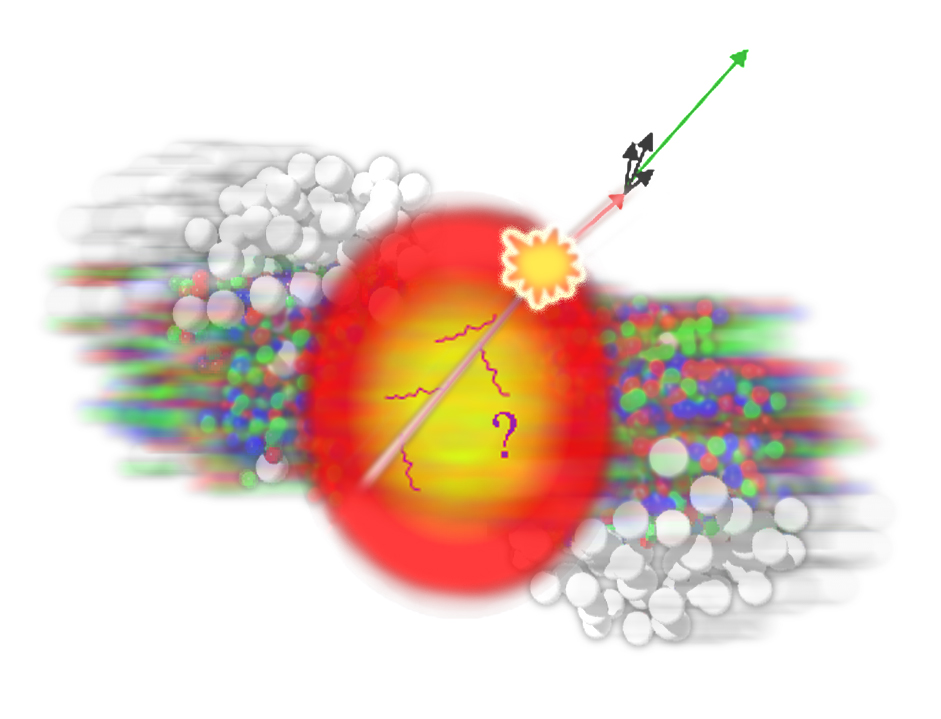
\includegraphics[width=0.9\linewidth]{jet-quenching.jpg}
\endminipage\hfill
\vspace*{-0.25cm}
\begin{itemize}
\item Monte Carlo simulation $\leftarrow$ my contribution
\end{itemize}
\vspace*{1cm}

\end{frame}

\section{Context}

\begin{frame}

%\frametitle{\small \flushleft HIC's, QGP's and jets}
%Heavy ion collisions, quark gluon plasma and jets,\\
%what we observe:
\minipage{0.5\textwidth}
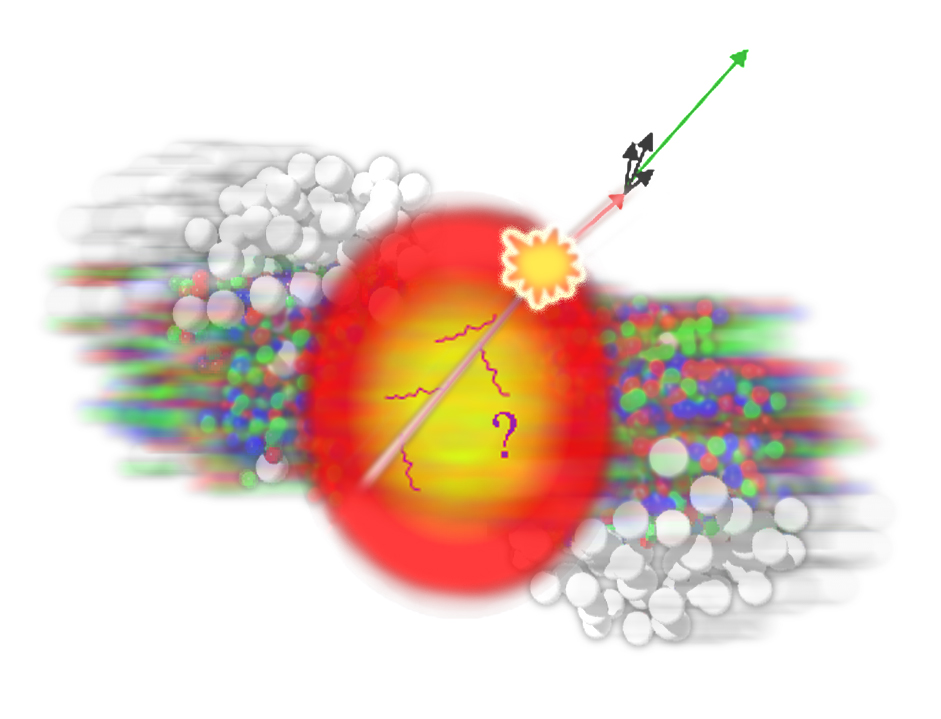
\includegraphics[width=0.9\linewidth]{jet-quenching.jpg}
\endminipage\hfill
\minipage{0.5\textwidth}
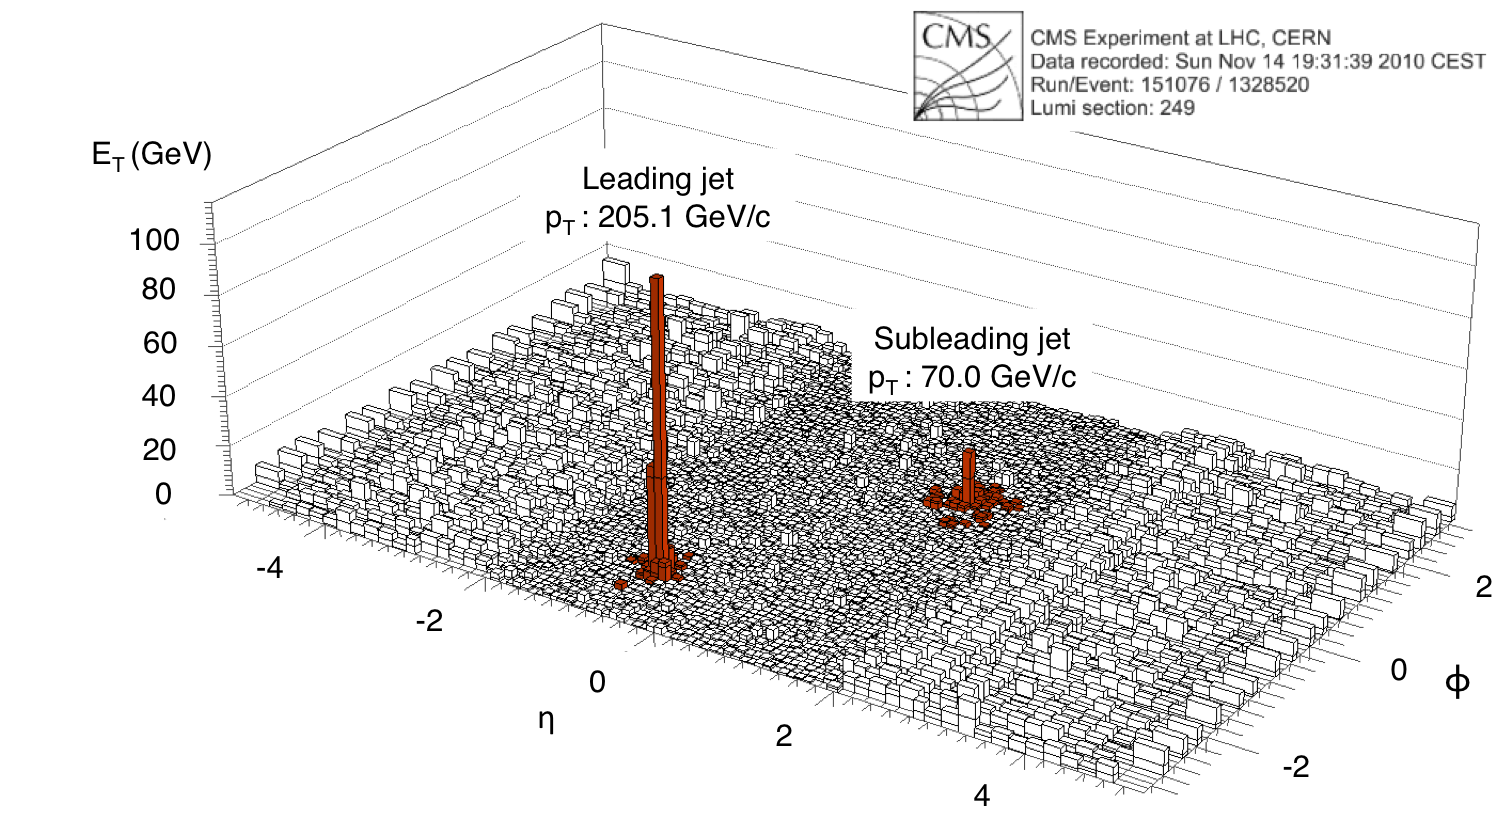
\includegraphics[width=1\linewidth]{CMS_JetQ.png}
\endminipage\hfill
%\begin{center}
%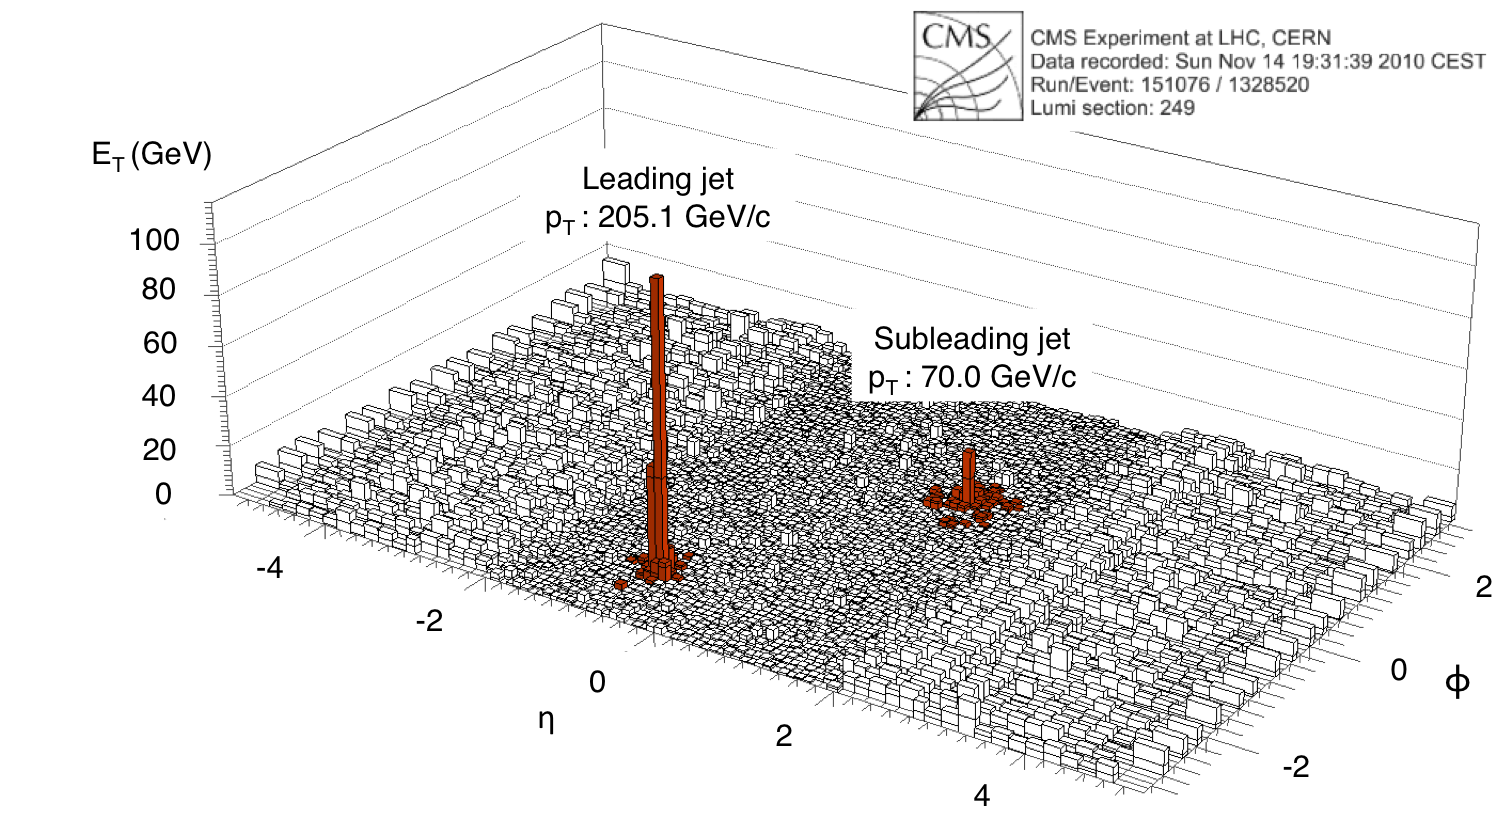
\includegraphics[width=1\linewidth]{CMS_JetQ.png}
%\end{center}
%Note: this picture is misleading.
%This is one of the findings, fluctuations
%are large enough to compete with jets
%travelling a different distance through the medium

%Di-jet asymmetry. 
Observation: jet loses energy in medium. Missing energy found among soft hadrons at large angles.% $\Rightarrow$ different from in vacuum jet evolution.
\begin{itemize}
\item Question 1: why large angles?
\end{itemize}


\end{frame}



\begin{frame}
 %\begin{textblock}{0.5}(0.001,0.001)
 % Test
 %\end{textblock}
%\vspace*{0.5cm}
%Heavy ion collisions, quark gluon plasma and jets,\\
%the stereotypical picture:
%\begin{center}
%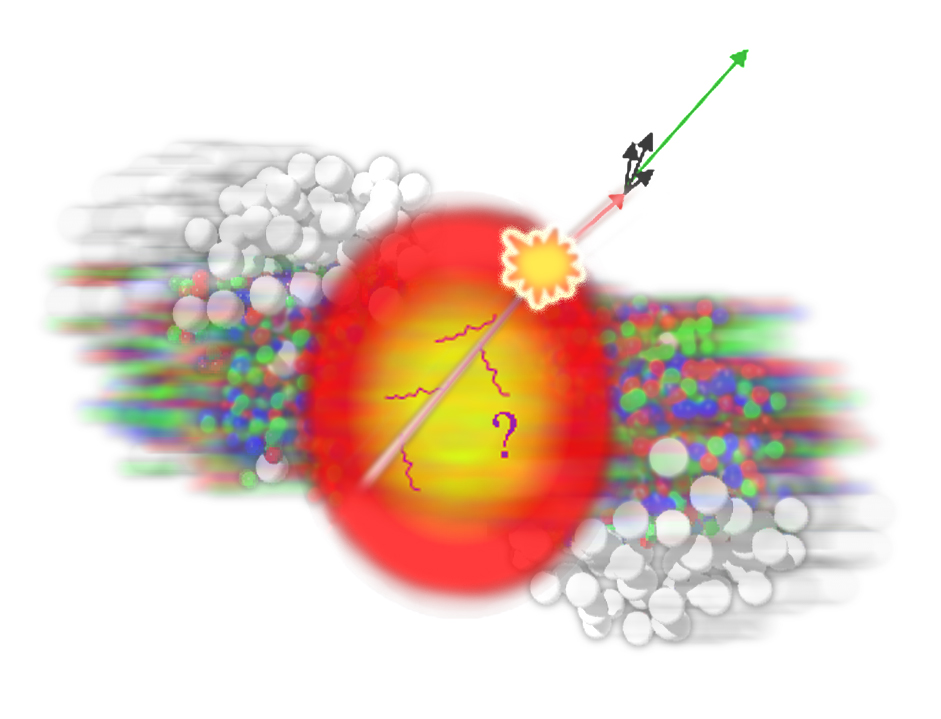
\includegraphics[width=0.45\linewidth]{jet-quenching.jpg}
%\end{center}
%Note: this picture is misleading.
%This is one of the findings, fluctuations
%are large enough to compete with jets
%travelling a different distance through the medium


Difference in energy loss, competition between geometry and fluctuations:

\vspace*{0.5cm}

\minipage{0.5\textwidth}
	\centering
	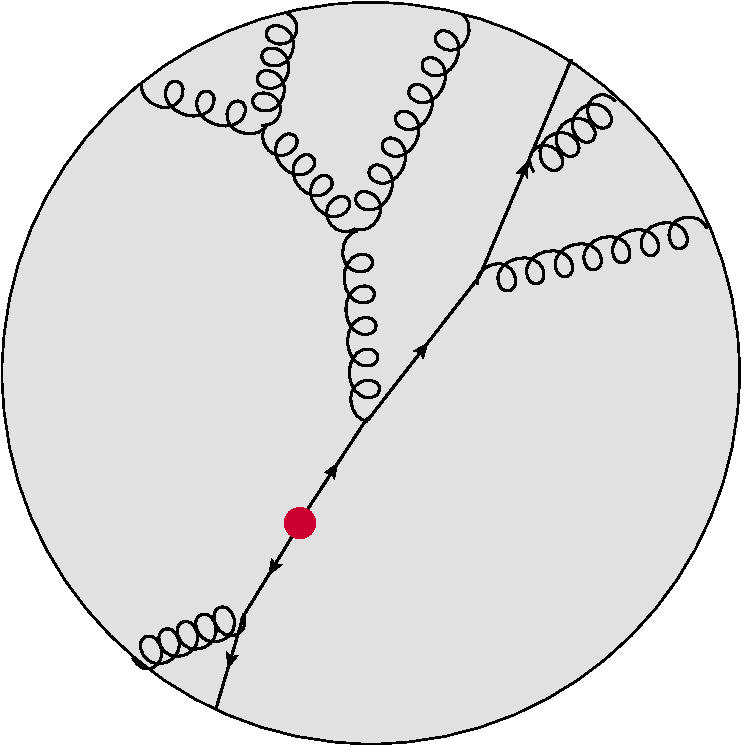
\includegraphics[width=0.7\linewidth, angle=180,origin=c]{Dijet_flucts1.pdf}
\endminipage\hfill
\minipage{0.5\textwidth}
	\centering
  	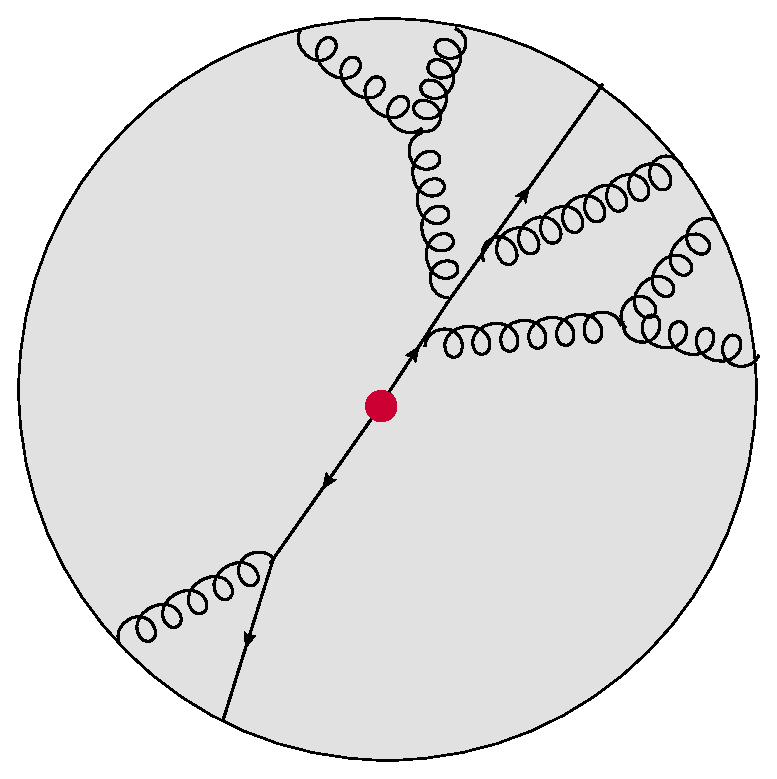
\includegraphics[width=0.7\linewidth, angle=180,origin=c]{Dijet_flucts2.eps}
\endminipage\hfill
\vspace*{1cm}

\begin{itemize}
\item Question 2: how large fluctuations?
\end{itemize}


\end{frame}



\section{Physical picture}

\begin{frame}[t]
\frametitle{Physical picture}
\begin{center}
\begin{tikzpicture}
    \node[anchor=south west,inner sep=0] (image) at (0,0) {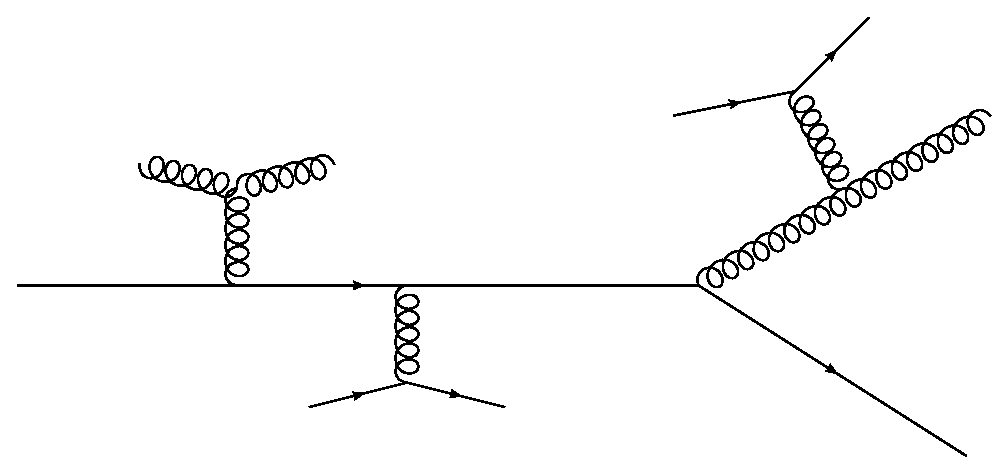
\includegraphics[width=0.6\textwidth]{scattering.eps}};
    \begin{scope}[x={(image.south east)},y={(image.north west)}]
        \draw[] (0.80,0.25) arc (-12:12:0.7);
        \node[] at (1, 0.85) {$\omega,k_\perp$};
        \node[] at (0.85, 0.4) {$\theta$};
        \draw[red,thick,dashed, <->] (0.95,0.05) -- (0.95,0.7);
        \node[red,right] at (0.95, 0.4){$\Delta x_\perp$};
        \draw[blue,thick, dashed,<->] (0.7,0) -- (0.95,00);
        \node[blue,below] at (0.85, 0){$\Delta t_f$};
    \end{scope}
\end{tikzpicture}
\end{center}

Source of energy loss: medium induced radiation.\\
~\\

\begin{itemize}
\item Scattering destroys quantum coherence
\end{itemize}


Formation time: ${\color{blue}\Delta t_f = \frac{\omega}{k_\perp^2}}$, from criterion $\lambda_\perp<\Delta x_\perp$.

%\frac{1}{k_\perp}<\frac{k_\perp}{\omega}\Delta t_f 

~\\
(Note: mostly gluon emissions $\Rightarrow$ consider only these.)
\end{frame}

\begin{frame}[t]
\frametitle{Physical picture}
\begin{center}
\begin{tikzpicture}
    \node[anchor=south west,inner sep=0] (image) at (0,0) {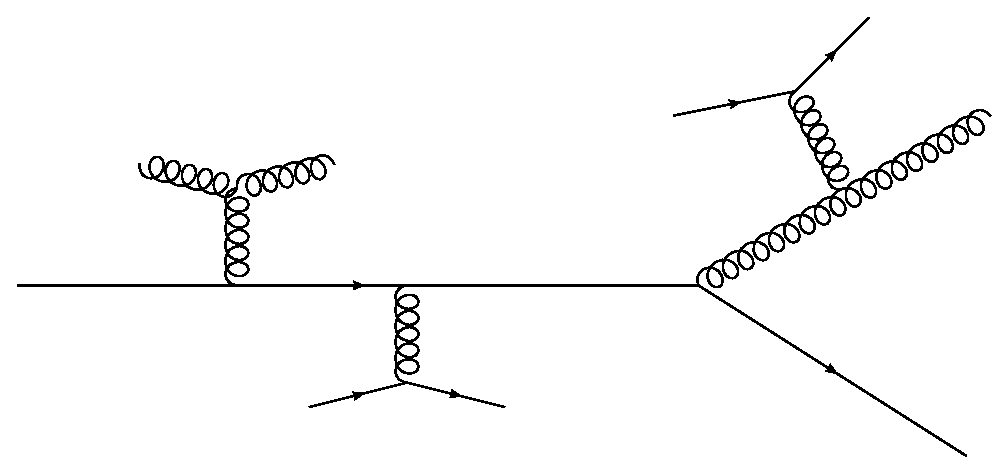
\includegraphics[width=0.6\textwidth]{scattering.eps}};
    \begin{scope}[x={(image.south east)},y={(image.north west)}]
        \draw[] (0.80,0.25) arc (-12:12:0.7);
        \node[] at (1, 0.85) {$\omega,k_\perp$};
        \node[] at (0.85, 0.4) {$\theta$};
        \draw[red,thick,dashed, <->] (0.95,0.05) -- (0.95,0.7);
        \node[red,right] at (0.95, 0.4){$\Delta x_\perp$};
        \draw[blue,thick, dashed,<->] (0.7,0) -- (0.95,00);
        \node[blue,below] at (0.85, 0){$\Delta t_f$};
    \end{scope}
\end{tikzpicture}
\end{center}

\begin{itemize}
\item Scattering gives broadening of transverse momentum
\end{itemize}

$\Delta t_f \gg $ mean free path $\gg$ Debye length\\ $\Rightarrow$  multiple scatterings lead to one emission \emph{and} scattering centers are independent \\ $\Rightarrow$ random walk \\
$\Rightarrow$  ${\color{blue} \langle k_\perp^2 \rangle \sim \hat{q}\Delta t }$, with $\hat{q}$ being the jet quenching parameter.

%\begin{center}
%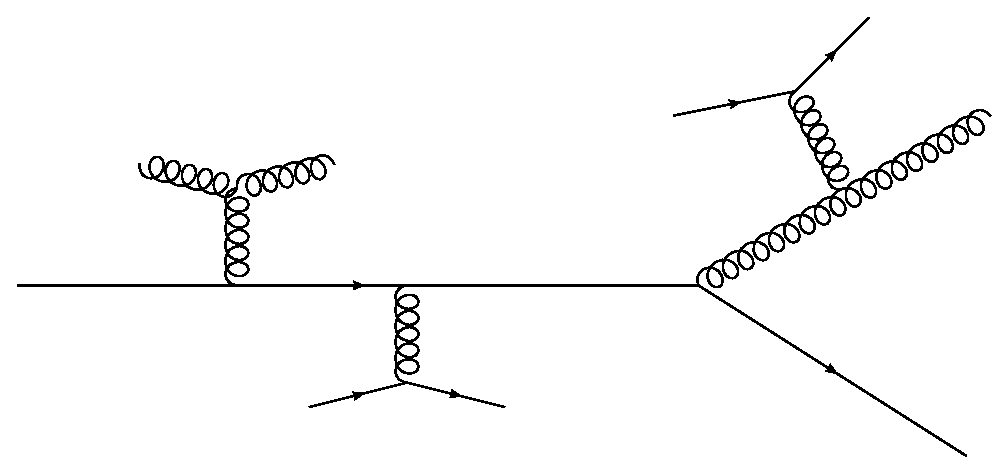
\includegraphics[width=0.5\linewidth]{scattering.eps}
%\end{center}

\end{frame}
\begin{frame}


\begin{center}
${\color{blue} \Delta t_f = \frac{\omega}{k_\perp^2}} \quad \quad \quad \quad \quad {\color{blue}\langle k_\perp^2 \rangle \sim \hat{q}\Delta t}$ 

\begin{tikzpicture}
\draw[thick, ->] (1,1) -- (1.4,0.6);
\draw[thick, ->] (4,1) -- (3.6,0.6);
\end{tikzpicture}
\end{center}
$$\Delta t_f \sim \sqrt{\frac{\omega}{\hat{q}}}$$
~\\
~\\
Angles: $\theta_f=\frac{k_\perp}{\omega} = \left( \frac{\hat{q}}{\omega^3} \right)^{1/4}$

$\Rightarrow$ we favour soft gluons at large angles!\\
~\\

BUT not the end of the story...
\end{frame}

\begin{frame}

Small $\omega$ gives small $\Delta t_f  \Rightarrow$  need to consider multiple branchings. Hardest scale for multiple branchings:
$$\omega_{br}= \bar{\alpha}^2 \hat{q}L^2.$$
\begin{flushright}
{\tiny ($\bar{\alpha}=\alpha_sN_c/\pi$) }
\end{flushright}

%Harder: not probable enough.

%Softer: not energetic enough.

Primary gluons emitted with $\omega_{br}$ can undergo democratic branchings (child gluons split energy $\sim$ equally).

\end{frame}

\begin{frame}[t]
\begin{center}
\begin{overpic}[width=0.65\linewidth]{democraticbranch.eps}
	\put(5,45){$E$}
	\put(59,49){$\omega \sim \omega_{br}$}
	\put(86,36){{\color{gray}$\omega \ll \omega_{br}$}}
	\put(46,76){$(1-z) \omega$}	
	\put(71,59){$z \omega$}
	\put(100,58){$T$}
	\put(96,76){$T$}
\end{overpic}
\end{center}
%\vspace*{-0.5cm}
%
Mechanism for energy loss:

\begin{itemize}
\small
\item $\mathcal{O}(1)$ of primary gluon emissions with $\omega \sim \omega_{br}$.
\item They then branch democratically, transporting away all energy.
\item Hence both energy loss and its fluctuations on the scale $\omega_{br}$.
\end{itemize}

\end{frame}


\begin{frame}[t]
\begin{center}
\begin{overpic}[width=0.65\linewidth]{democraticbranch.eps}
	\put(5,45){$E$}
	\put(59,49){$\omega \sim \omega_{br}$}
	\put(86,36){{\color{gray}$\omega \ll \omega_{br}$}}
	\put(46,76){$(1-z) \omega$}	
	\put(71,59){$z \omega$}
	\put(100,58){$T$}
	\put(96,76){$T$}
\end{overpic}
\end{center}

Time between branchings $\gg$ formation time\\
 $\Rightarrow$ branchings are independent\\
  $\Rightarrow$ Markov process
\end{frame}


\section{Markov process}
\begin{frame}
\frametitle{Markov process}


Branching rate from BDMPS-Z spectrum:
$$\frac{\mathrm{d}^2 P(z,\tau)}{\mathrm{d}z\mathrm{d}\tau}=\frac{K(z)}{2 \sqrt{x}}$$
\begin{itemize}
\item $\tau=\frac{\text{propagation time}}{\text{democratic branching time for leading particle}}$,  $\quad x=\frac{\omega}{E}$
\item Splitting kernel: $K(z)=\frac{[1-z(1-z)]^{5/2}}{[z(1-z)]^{3/2}} \approx  \frac{1}{[z(1-z)]^{3/2}}$
\end{itemize}
~\\


For the energy spectrum we consider
$D(x,\tau)\equiv xn(x,\tau)$, for the fluctuations we also need $D^{(2)}(x,x'\tau)\equiv xx'n^{(2)}(x,x',\tau)$.

\begin{center}
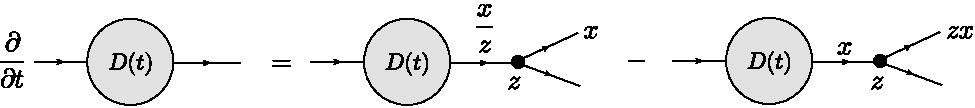
\includegraphics[width=1\linewidth]{RateEq_D.pdf}
\end{center}

%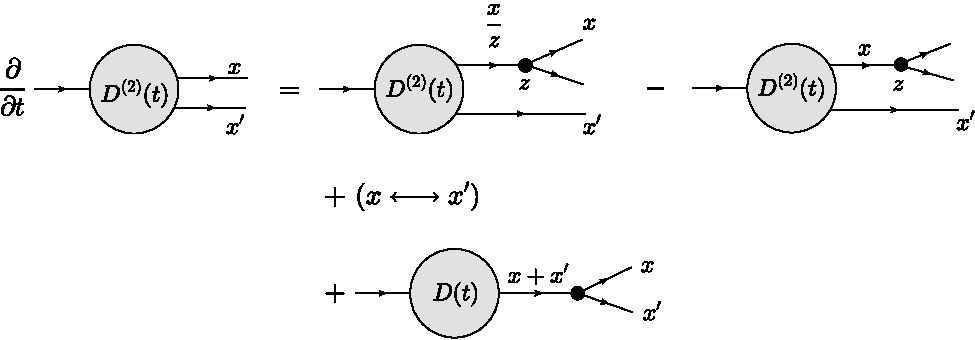
\includegraphics[width=0.8\linewidth]{RateEq_D2.pdf}

%$\party{}{\tau}D(x,\tau)=\int \mathrm{d}z\, K(z) \left[\sqrt{\frac{z}{x}} D\left(\frac{x}{z},\tau\right)- \frac{z}{\sqrt{x}}D(x,\tau)  \right]$
\end{frame}


\begin{frame}[t]
Analytic result, simple kernel:
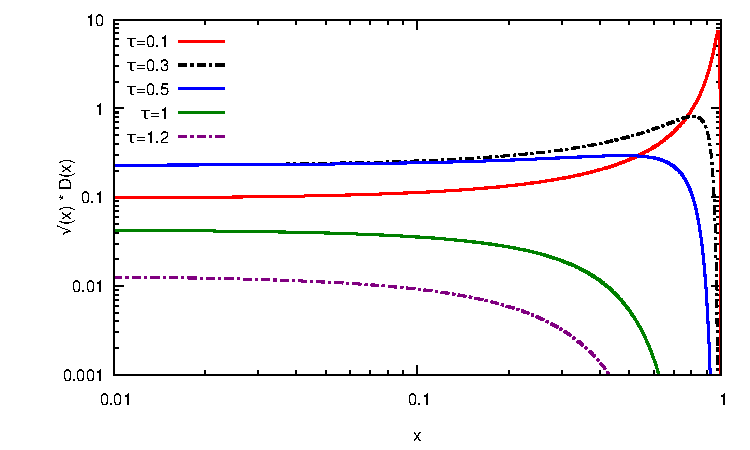
\includegraphics[width=0.9\linewidth]{plotD.pdf}

\begin{itemize}
\item $D(x,\tau)=\frac{\tau}{\sqrt{x}(1-x)^{3/2}}\exp\left(-\frac{\pi \tau^2}{1-x}\right)$. 
\item $\int_0^1 \mathrm{d}x\, D(x,\tau) = e^{-\pi\tau^2}$ $\Rightarrow$ energy decreasing in time. 
\item Formally: condensate at $x=0$. Physically: thermalization.
%\item At small $\tau$, loss $\simeq \pi \omega_{br}$. 
%\item $D^{(2)}(x,x'\tau)$ used to find fluctuations. To order $\tau^4$:
% $$\sigma_\epsilon(\tau)\simeq \langle \epsilon(\tau)\rangle/\sqrt{3}$$.
\end{itemize}
\end{frame}

\begin{frame}[t]
Analytic result, simple kernel:
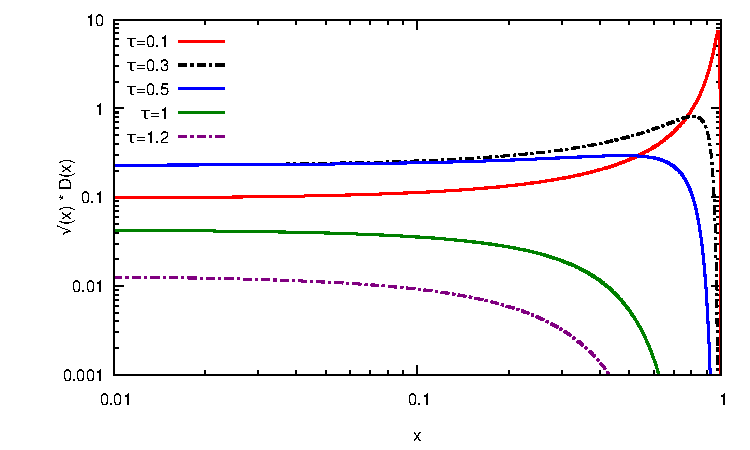
\includegraphics[width=0.9\linewidth]{plotD.pdf}

\begin{itemize}
%\item $D(x,\tau)=\frac{\tau}{\sqrt{x}(1-x)^{3/2}}\exp\left(-\frac{\pi \tau^2}{1-x}\right)$
%\item $\int_0^1 \mathrm{d}x\, D(x,\tau) = e^{-\pi\tau^2}$ $\Rightarrow$ energy decreasing in time. 
%\item Formally: condensate at $x=0$. Physically: thermalization.
\item At small $\tau$, loss $\simeq \pi \omega_{br}$. 
\item $D^{(2)}(x,x'\tau)$ used to find fluctuations. To order $\tau^4$:
 $$\sigma_\epsilon(\tau)\simeq \langle \epsilon(\tau)\rangle/\sqrt{3}$$.
\end{itemize}
\end{frame}


\section{Monte Carlo simulation}

\begin{frame}
\begin{center}
New work: Monte Carlo simulation\\
~\\
\url{https://github.com/gsoyez/SimpleMediumBranching}
\end{center}

\end{frame}



\begin{frame}
\frametitle{Monte Carlo simulation}

Result: full kernel $\Rightarrow$ less efficient branching\\
~\\

%\vspace*{1cm}


\minipage{0.5\textwidth}
\centering
\small $\sqrt{x} D(x)$
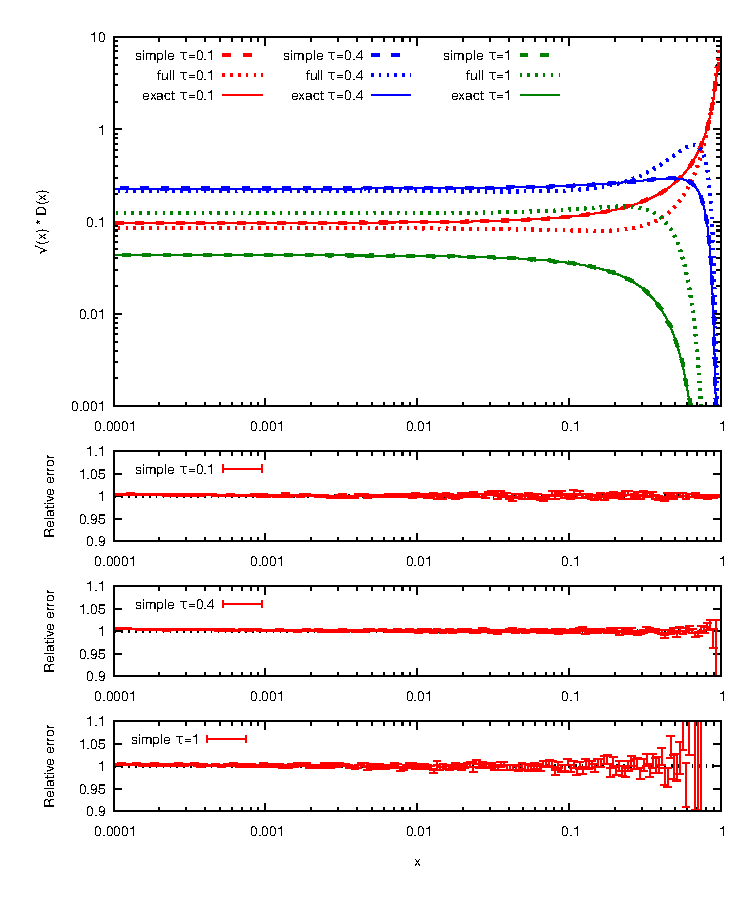
\includegraphics[width=1\linewidth]{times.pdf}
\endminipage\hfill
\minipage{0.5\textwidth}
%\centering
\small 

Simple splitting kernel, numerical versus analytic:
\begin{itemize}
\item Good agreement overall
\item Small x bias $<$ 1\%
\end{itemize}

Corrections from the full splitting kernel:
\begin{itemize}
\item Leading peak still present at $\tau=0.5$
\item Less energy lost at $\tau=1$
\end{itemize}


Recall:

Simple $K(z)=\frac{1}{[z(1-z)]^{3/2}}$


Full $K(z)=\frac{[1-z(1-z)]^{5/2}}{[z(1-z)]^{3/2}}$


\endminipage\hfill


\end{frame}


\begin{frame}
\frametitle{Monte Carlo simulation}

Result: full kernel $\Rightarrow$ less efficient branching\\
~\\

%\vspace*{1cm}


\minipage{0.5\textwidth}
\centering
\small $\sqrt{x} D(x)$
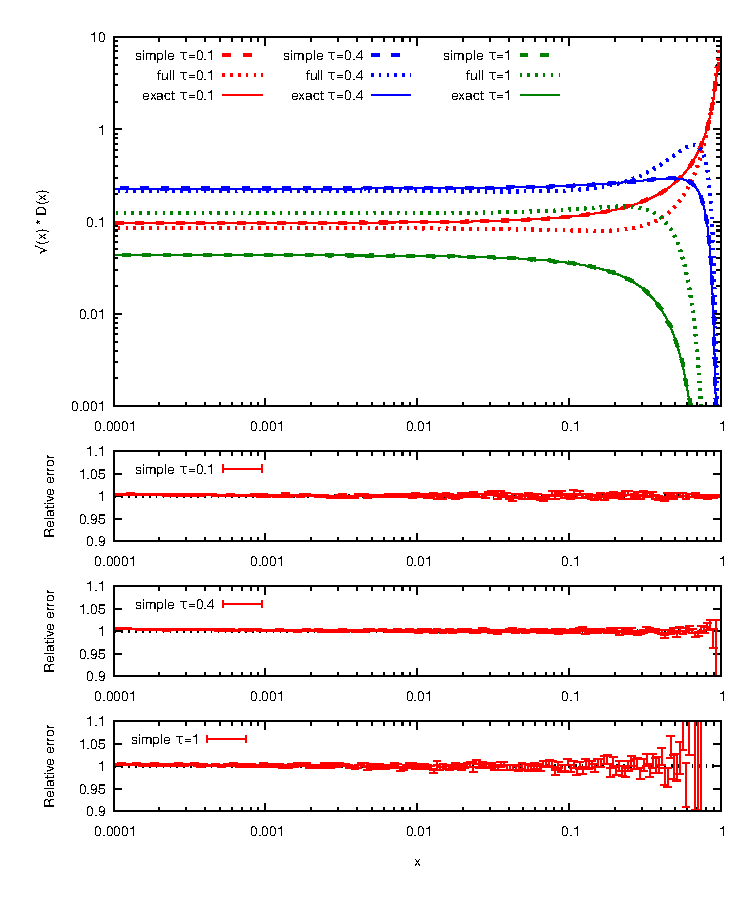
\includegraphics[width=1\linewidth]{times.pdf}
\endminipage\hfill
\minipage{0.5\textwidth}
\centering
\small $x D^2(x,x)$
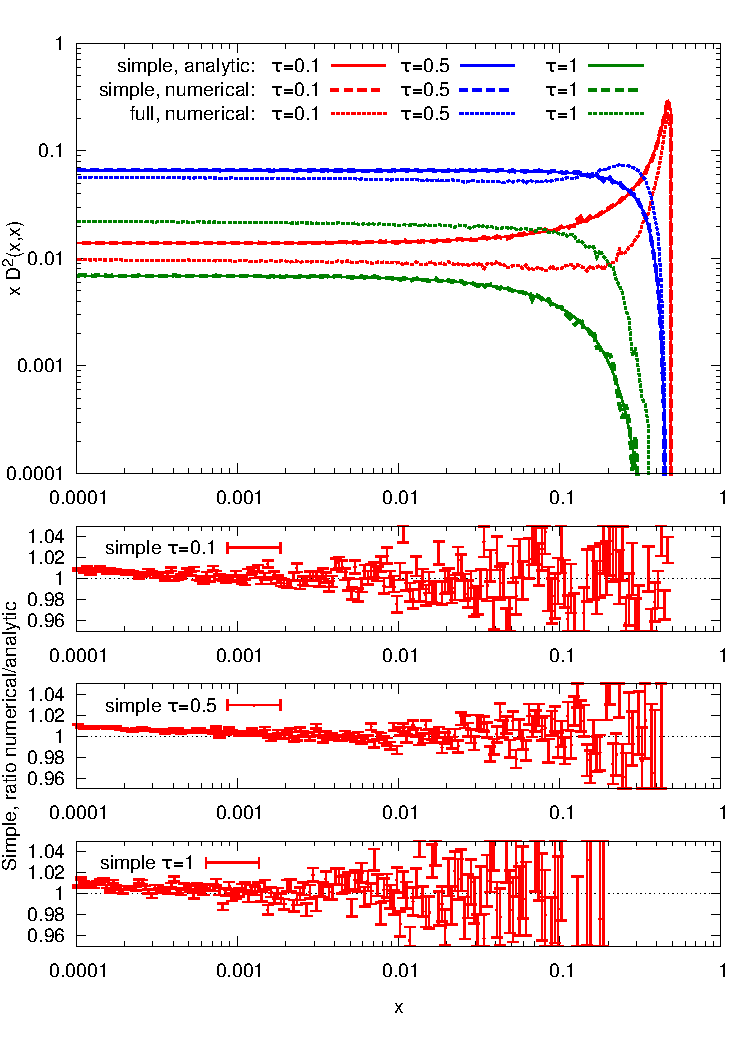
\includegraphics[width=1\linewidth]{D2.pdf}
\endminipage\hfill


\end{frame}



\begin{frame}
Energy loss and its fluctuations - new result!
{\centering
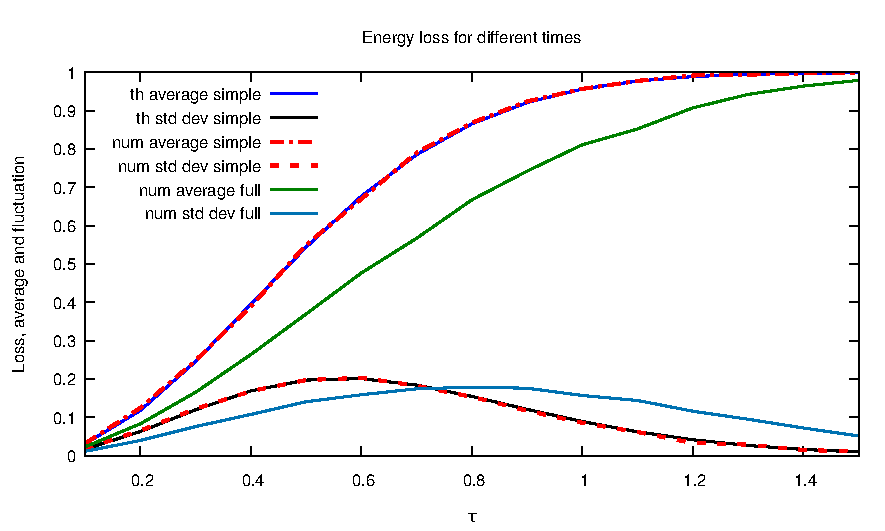
\includegraphics[width=1\linewidth]{energyloss.pdf}
}
Full kernel $\Rightarrow$ shifted in $\tau$ but same qualitative picture.
\end{frame}



\section{Outro}
\begin{frame}

%Maybe something about future work, discussion etc. I should probably have the thesis itself in a pdf viewer for easy reference in case of questions.

Summary:

\begin{itemize}
\item Democratic branchings $\Rightarrow$ energy found at large angles
\item Prediction: large fluctuations in energy loss
\item My contribution: Monte Carlo simulation
\item First results for full kernel: same qualitative behaviour, quantitative differences
\end{itemize}
~\\
\center THE END\\
~\\
Questions?

\end{frame}

\end{document}